Our approach includes the additional parameter of scent as a factor.
Biology supports our claim due to the fact that some materials are decomposed over time.
This decomposition has side effects, namely the production of certain gasses,
which can be detected by a variety of sensors due to their multiple characteristics of density and conductivity.
%Gasses can have multiple characteristics - hence a variety of sensors able to detect gasses exist.
We are interested in the gasses easily detectable by humans - namely the ones with a characteristic smell.
%Humans have a hard time detecting the odour-less ones.

Our system is composed of four main components, a \textit{sensory layer}, a \textit{communication module},  a \textit{	data layer}, and a \textit{data consumer}. 
%\begin{itemize}
%\item sensory layer: responsible of producing information, placed directly on the bin.
%\item communication module: responsible of sending such information.
%\item data layer (the cloud): this component stores the data and makes it available.
%\item data consumer (android):  this client shows information to the end user on request
%\end{itemize}

\subsection{Sensory layer and Communication module}
The sensory layer has two sensors (figure \ref{fig:sensors}) and one communication device. The sensors detect the state of the bin.
Our approach relies on two kinds of information related to the state of the bin: smell and fill level.
For this reason, the sensory part of the system is of key importance, since it enables the information to be perceived and registered by the system.
An odor detection sensor is able to capture volatile organic compounds (VOCs) and other gases, typical by products of food decomposition, commonly associated with bad smell. 
Some examples are Hydrogen Sulphide (\ce{H_{2}S}), Ammonia(\ce{NH_3}), Toluene (\ce{CH_3}) and others.
The smartbin sends the raw values of VOC concentration to the data layer.

The other type of sensor is a ultrasonic distance measurement unit. This is used to get the distance to the bottom of the bin.
This type of information is processed in the sensory layer to reflect the amount of thrash filled in the bin.

The raw values are then processed and formatted into something understandable for our data layer.
The last step is to send the values using the communication module. In this study a WiFi adapter was used.

\begin{figure}
\centering
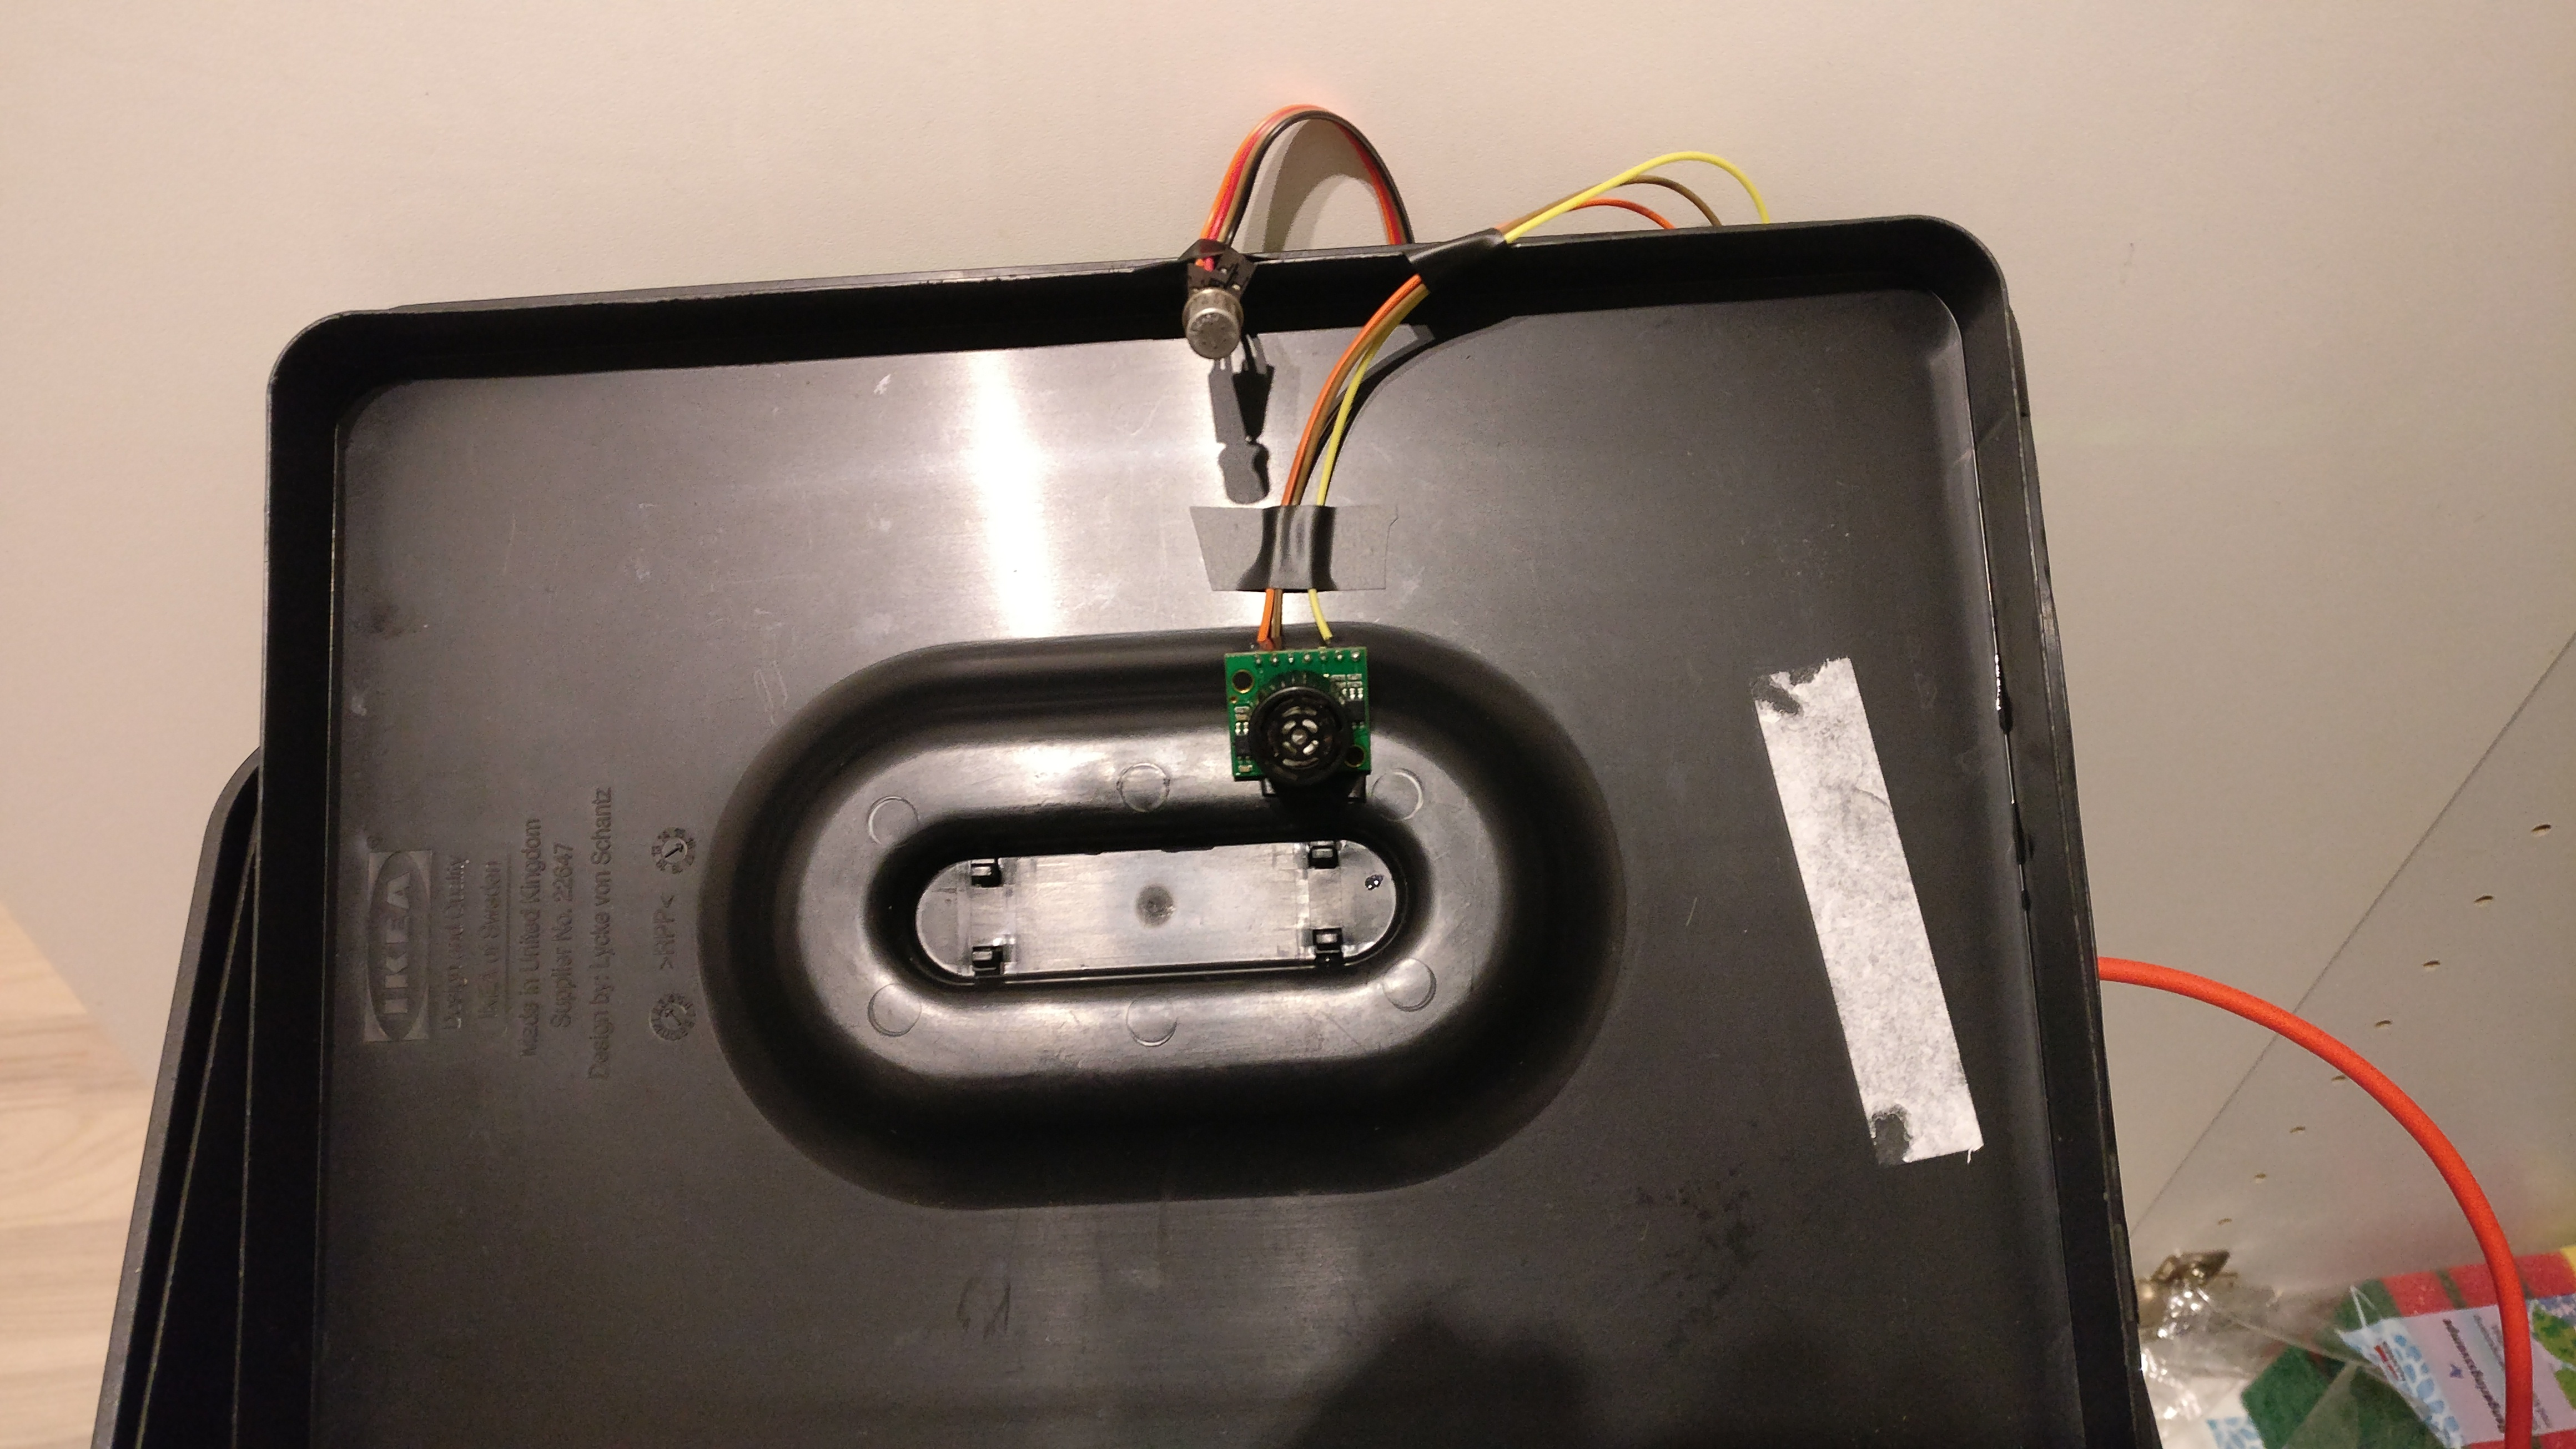
\includegraphics[scale=.05]{img/IMG_20161130_163302}
\caption{The sensors.}
\label{fig:sensors}
\end{figure}

\subsection{Data layer}
The data layer is a simple restfull webservice for collecting the data and storing it in a database, making it accessible to potential consumers.
The service supports two types of entities. The SmartBins and the contexts.
In short a SmartBin represents the hardware instance of a smartbin, this includes information such as location expressed as coordinates, unique identifier, 'calibration' which is the intial air quality level (in "clean" air, a value to which compare later measurements) and meta information about the last associated context.
This ensures that status of every bin is readily available without having to traverse the contexts.
The contexts model a snapshot of a bins state at a given time.

\subsection{Data Consumer}
The consumer in our case is an android client, but could just as easily have been any other platform able to connect to the internet and present content.

Our client can work in two separate modes: either as an android application or simply as an ambient display(single bin mode).

On the android application it is possible to manage multiple bins and get an overview of the last values measured by the system.

The ambient display is much more simple, it just displays a color of a shade from blue to red depending on the scent level.

In our system we use an android phone to run in both modes, so pressing on the screen even in ambient display mode will give the user the extra functionality of knowing trash level and emission level.

Ideally the ambient display can be placed in a strategic location inside the house, for example by the door or on the fridge, where people can be reminded of the trash status and act accordingly.

Figure \ref{fig:interaction} shows an example of interaction with the ambient display.

\begin{figure}
\centering
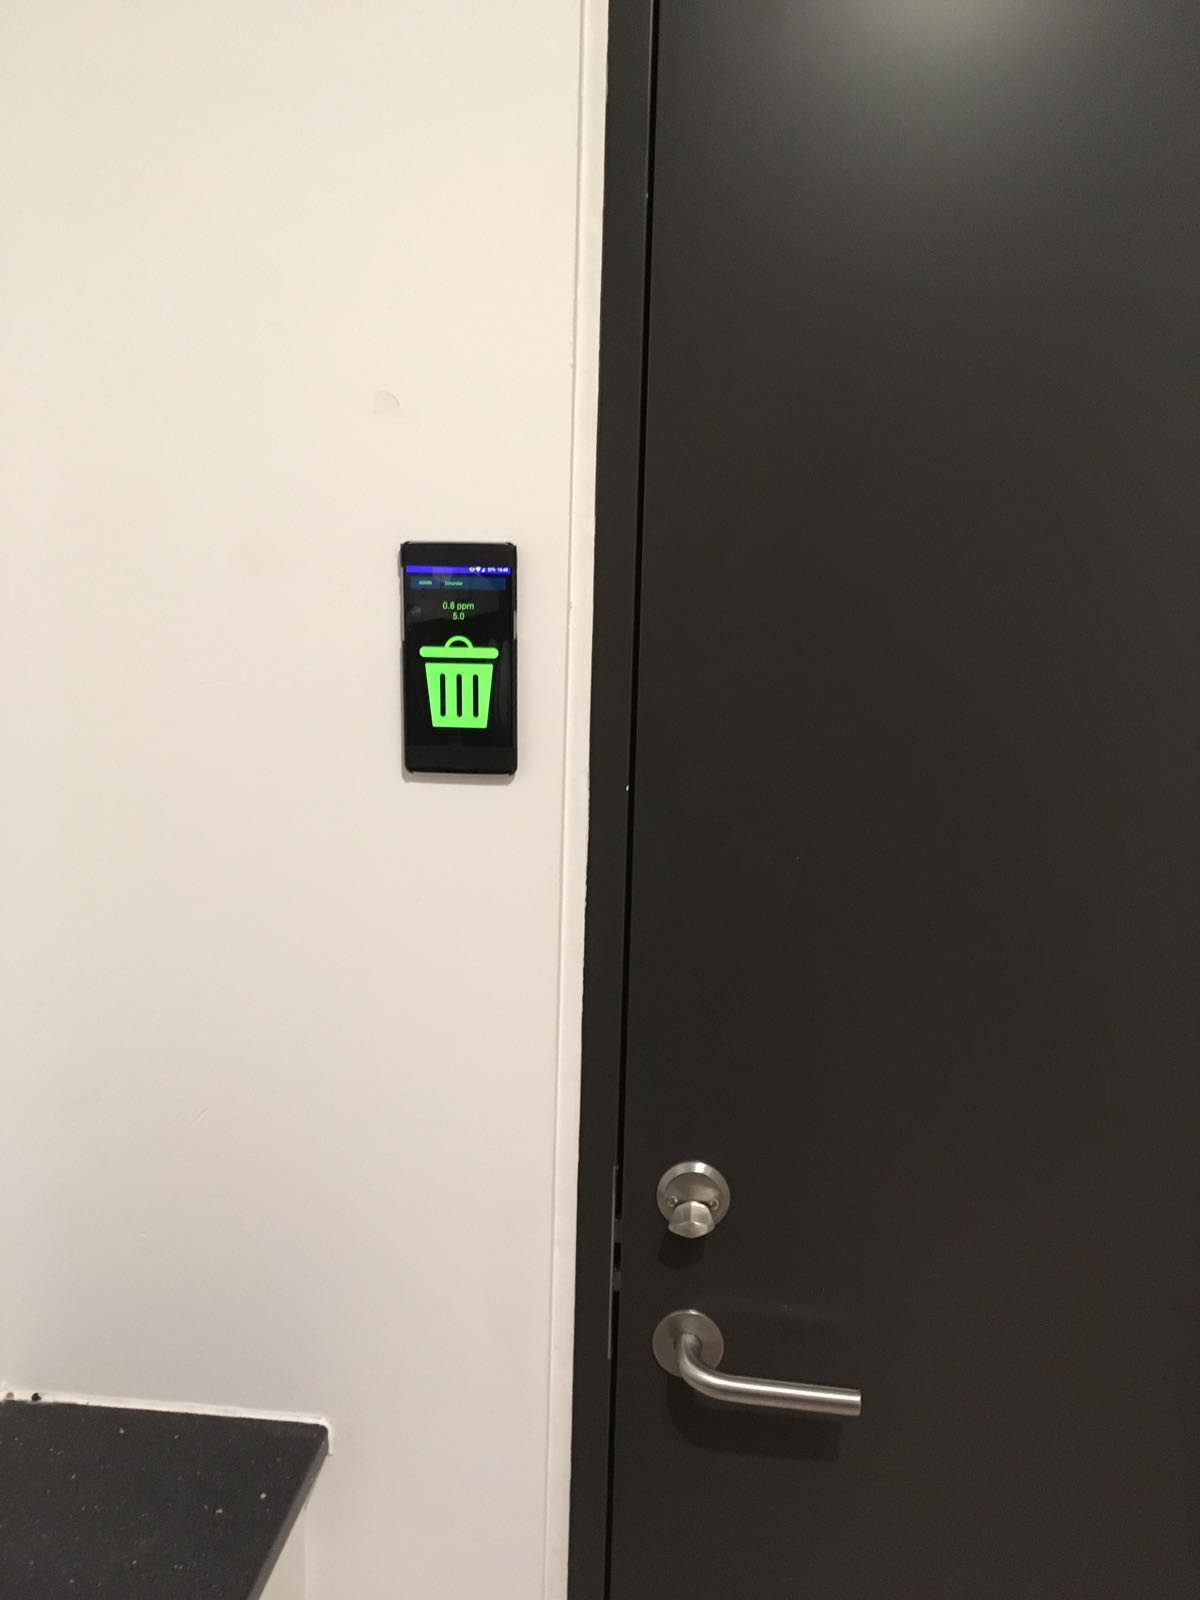
\includegraphics[scale=.05]{img/IMG-20161130-WA0000}
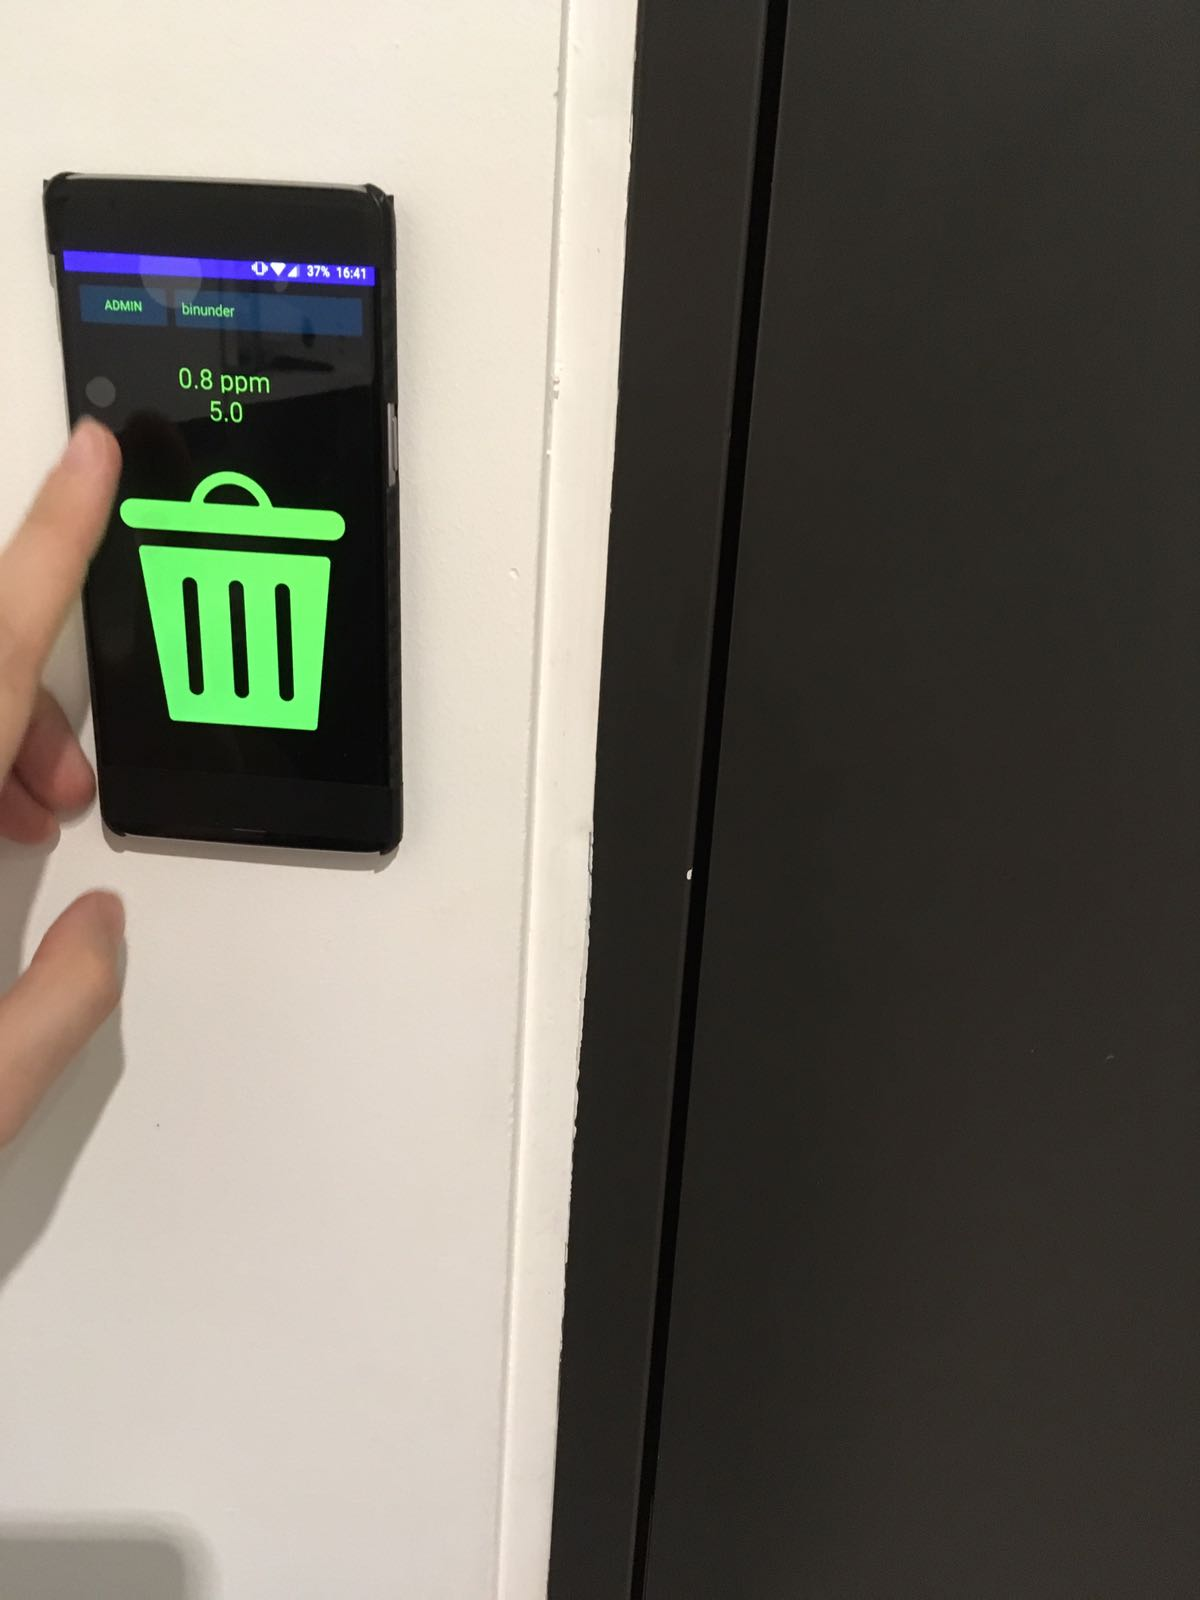
\includegraphics[scale=.05]{img/IMG-20161130-WA0004}
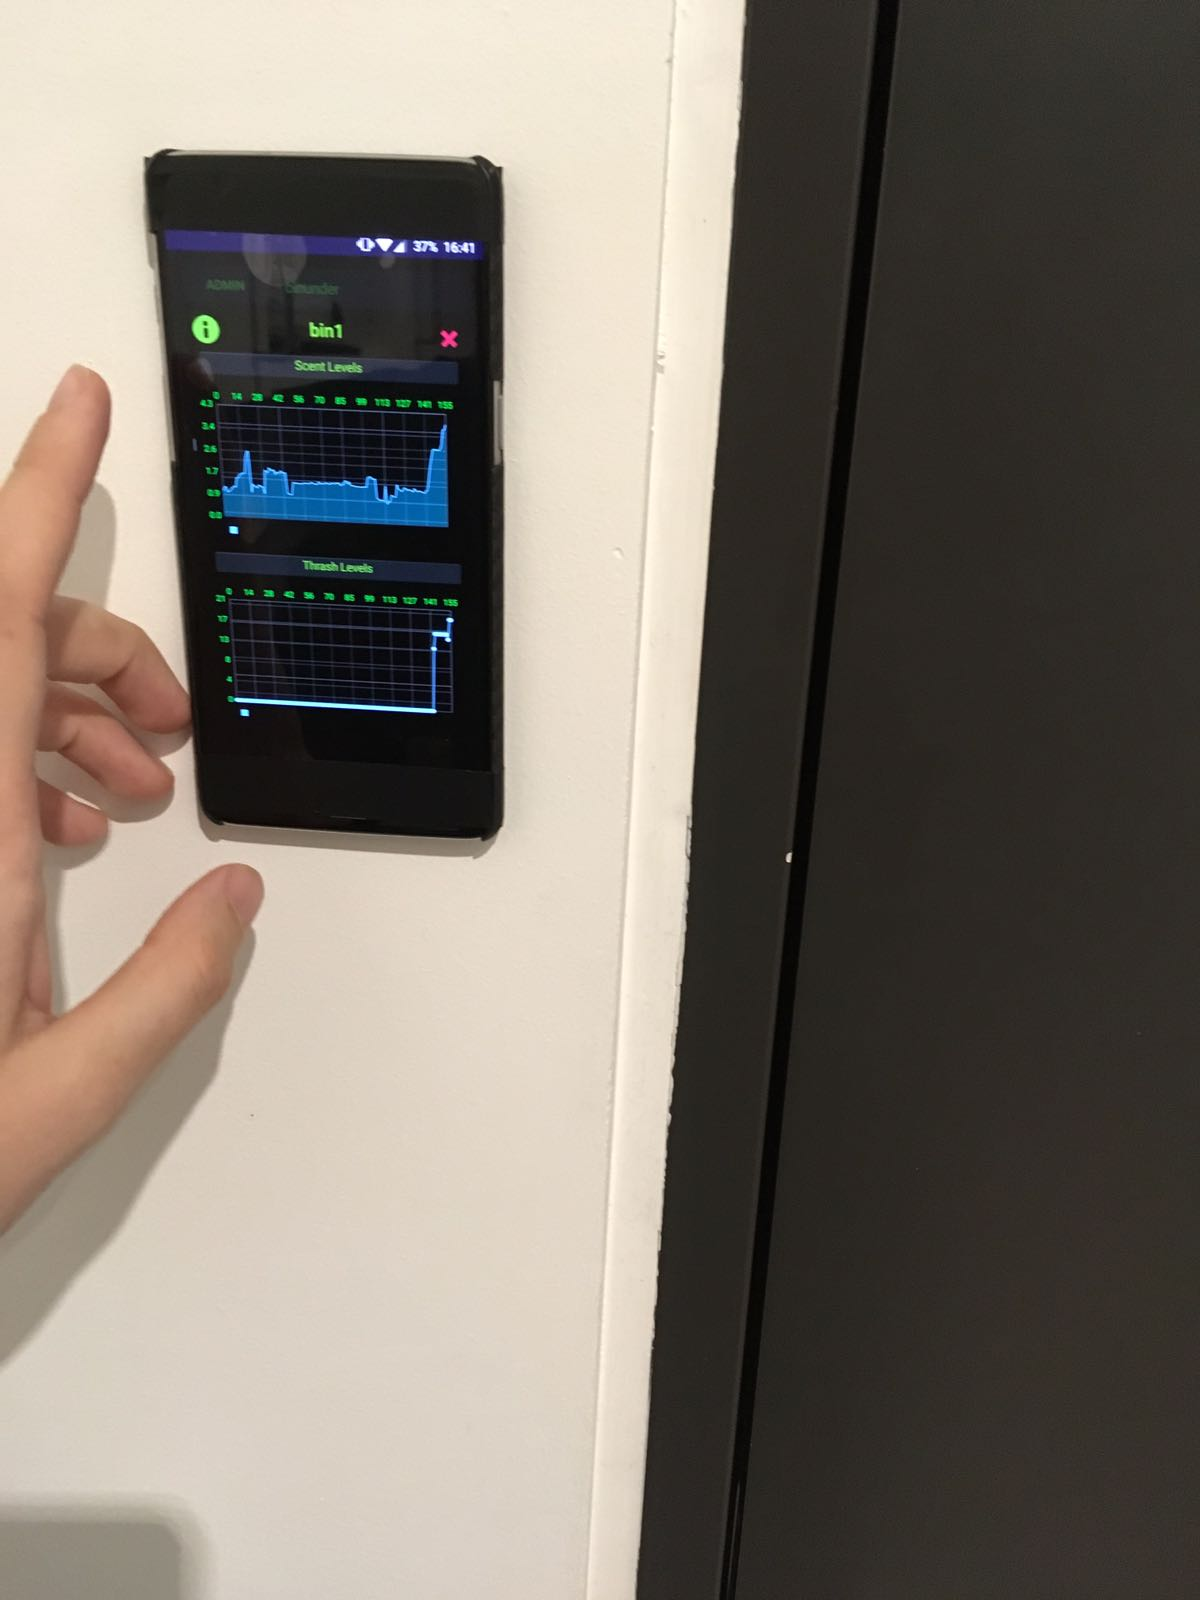
\includegraphics[scale=.05]{img/IMG-20161130-WA0002}
\caption{Interaction with ambient display}
\label{fig:interaction}
\end{figure}